%package obligatoire : type de document
\documentclass[a4paper,12pt,twoside]{book}

% encodage
\usepackage{fontspec}

% Annexes (à déclarer avant hyperref)
\usepackage{appendix}

% le package hyperref avec des options, si en local
\usepackage[pdfusetitle, pdfsubject ={Mémoire TNAH}, pdfkeywords={les mots-clés}]{hyperref}

%il faut mettre au moins une langue
\usepackage[english,french]{babel}
% Commande personnalisée pour la typographie des langues
\newcommand{\langue}[1]{\emph{#1}}

% configurer le document selon les normes de l'école
\usepackage[margin=2.5cm]{geometry} %marges
\usepackage{setspace} % espacement qui permet ensuite de définir un interligne
\onehalfspacing % interligne de 1.5
\setlength\parindent{1cm} % indentation des paragraphes à 1 cm

% Table des matières
\addto\captionsfrench{
\renewcommand*\contentsname{Contenu de la documentation}
}
\usepackage[nottoc]{tocbibind}% Pour ajouter la biblio à la TDM sans numérotation de chapitre

% bibliographie
\usepackage[backend=biber, sorting=nyt, style=enc,maxbibnames=10]{biblatex}
\addbibresource{biblio.bib}

%\nocite{*}

% Sigles et acronymes
\usepackage[automake,acronym,toc]{glossaries}
\makeglossaries
\newacronym{cds}{CdS}{Constance de Salm}
\newacronym{dahn}{DAHN}{Digital Edition of historical manuscripts}
\newacronym{dhi}{DHIP}{Deutsches Historisches Institut Paris}
\newacronym{fud}{FuD}{Die Virtuelle Forschungsumgebung für die Geistes- und Sozialwissenschften}
\newacronym{htr}{HTR}{\textit{Handwritten Text Recognition}}
\newacronym{Segmonto}{SegmOnto}{SegmOnto~: A Controlled Vocabulary to Describe the Layout of Pages}

% Images
\usepackage{graphicx}

% Citations
\usepackage{csquotes}

% DOCUMENT
\begin{document}
	
	\tableofcontents
	
	\chapter*{Présentation}
	\addcontentsline{toc}{chapter}{Présentation}% Ajoute à la table des matières sans numérotation
	
		\section*{Contexte}
		\addcontentsline{toc}{section}{Contexte}
		Constance de Salm (1767-1845), femme de lettres française, a entretenu une vaste correspondance à partir de son mariage avec de nombreux intellectuels en Allemagne, en France, en Russie.

		Le projet de publier numériquement sa correspondance est né de l'intérêt pour les relations entre noblesses française et allemande au sein du \gls{dhi}. Il en a résulté la production d'un site \textit{Wordpress} adossé au système de base de données \href{https://fud.uni-trier.de/}{\gls{fud}}. Les notices de plus de 11000 lettres, publiées sur le site \href{https://constance-de-salm.de}{constance-de-salm.de}, associent la reproduction numérique des documents manuscrits (lettres, copies, brouillons, recueils) avec leurs métadonnées descriptives, ainsi qu'une transcription de la première ligne de chaque lettre.

		\section*{Objectifs}
		\addcontentsline{toc}{section}{Objectifs}
		L'objectif du stage consiste à mettre en place un flux de production automatisé pour l'édition des lettres au format XML-TEI. On s'appuiera pour cela sur les instruments et la documentation produits dans le cadre du projet \gls{dahn}, fondé sur l'édition de la correspondance de Paul d’Estournelles de Constant (1852-1924)\footcite{chiffoleauDAHNProject}.
		
		Il s'agit en particulier d'identifier les points de difficultés que posent le traitement de ce vaste corpus tant du point de vue de la transcription automatisée des documents que du point de vue de leur encodage au format TEI. Il serait notamment souhaitable, au terme du stage de disposer d'un flux de production pour l'édition d'un volume de recueil de lettres.
			
	\chapter{Reconnaissance automatique des écritures manuscrites}
		
		\section{Problématique}
		Quatre à cinq mains différentes ont été repérées jusqu'à présent dans la correspondance de \gls{cds} (mais aucune enquête paléographique complète n'a été menée). Cette variété des écritures est un problème majeur pour l'automatisation des transcriptions.
		
		Deux pistes méthodologiques se dessinent~:
		\begin{enumerate}
			\item Rassembler dans un premier temps des lettres qui sont de la même main, pour voir quels sont les résultats du modèle entraîné par H.~Souvay lors d'un précédent stage\footcite{souvayCorrespondanceConstanceSalm2021}~;
			\item Reprendre un modèle déjà entraîné à travailler sur plusieurs mains~; c'est l'option qui été privilégiée par le projet Lectaurep\footcite{chagueCreationModelesTranscriptiona}).
		\end{enumerate}
				
		\section{Choisir un corpus d'entraînement}
			Les recueils de lettres constituent la part du corpus la plus normée sur le plan de l'écriture et de la mise en page, leur qualité de conservation assurant en outre de bonnes conditions à la reconnaissance d'écriture. La distribution des mains y est variable selon les tomes :
		\begin{enumerate}
			\item Le premier volume\footcite{salmCorrespondanceGeneraleSecondea} présente une grande variété de mains s'enchaînant fréquemment les unes aux autres~;
			\item Le deuxième volume\footcite{salmCorrespondanceGeneraleSeconde}  présente en revanche une meilleure cohérence paléographique : la même main peut se suivre sur un bon nombre de pages consécutives, facilitant l'entraînement d'un modèle sur une écriture particulière. Nous avons repris ce volume, en partie utilisé par H. Souvay pour ses tests, afin de constituer un premier sous-corpus paléographiquement cohérent~;
			\item Le troisième volume\footcite{salmCorrespondanceGeneraleSecondeb}, où les mains du deuxième volume se retrouvent largement et a pu être joint au précédent.
		\end{enumerate}
	
			\subsection{Main 1}
			Nous avons établi une liste de 30 images (soit 30 doubles pages) au sein du 2e et du 3e volume attestant une écriture homogène que nous dénommons \textit{Main 1}. Nous avons pour cela sélectionné les lettres afin de ne travailler que sur un seul type d'écriture, sachant que les changements de main interviennent souvent en milieu de page. Quelques corrections de la main de \gls{cds} apparaissent ponctuellement.
		
			\subsection{Écriture de \gls{cds}}
			Le site ne publie aucune lettre originale de la main de \gls{cds}, mais 52 brouillons (\textit{Entwurf})\footnote{Le dépouillement se trouve dans le fichier \textsf{./htr/mains/brouillonsCDS.md}}.
		
			Entraîner un modèle de reconnaissance sur cette écriture supposerait un travail délicat de transcription pour une écriture particulièrement cursive (compter environ deux semaines pour disposer d'une bonne vingtaine de pages), mais l'investissement peut en valoir la peine.
		
		\section{Segmentation et annotation des zones d'écriture}
			Nous avons procédé à une première expérience de transcription sur le sous-corpus \textit{Main 1} avec le logiciel e-Scriptorium installé localement.
        
            \subsection{Typer les régions d'écriture}
            Le typage est utile en ce qu'il permet de traiter de manière différentielle des régions et des lignes afin de les affecter à des éléments distincts de l'arborescence XML-TEI qu'il faudra construire.
            
            Il faut donc réfléchir aux besoins de cette transformation vers le format TEI. Les \textit{Guidelines} de l'édition de correspondance du projet DAHN permettent de guider cette réflexion\footcite{chiffoleauCorrespondenceGuidelines2022}. Par ailleurs, F.~Chiffoleau a formulé une ontologie pour les régions et lignes des écrits de correspondance en langue française pour le XXe siècle \footcite{chiffoleauCorrespondanceLangueFrancaise2021} dans le cadre du projet \gls{Segmonto}\footcite{gabaySegmOntoCommonVocabulary2021}.
				        
	        Cetaines régions peuvent être directement appliquées :
			\selectlanguage{english}
			\begin{itemize}
				\item \textbf{Main}
				\item \textbf{Title}
				\item \textbf{Signature}: salutation and signature of the sender;
				\item \textbf{Letterhead}
				\item \textbf{Numbering}
				\item \textbf{Salute}
				\item \textbf{Dateline}: place and date of writing for the letter.
			\end{itemize}
			\selectlanguage{french}
			
			Il pourrait être pertinent de modifier l'usage de :
			\selectlanguage{english}
			\begin{itemize}
				\item \textbf{Additions}: \langue{cette catégorie est utilisée ailleurs dans \gls{Segmonto}, pour les documents administratifs			\selectlanguage{french}\footcite{chagueDocumentsAdministratifsXIXe2021}~; elle intervient dans le traitement du document postérieurement à sa rédaction. Cette pertinence reste cependant à confirmer. Cette catégorie pourrait également s'appliquer aux rubriques~:}
				\begin{figure}[!h]
					% !h ancre l'image dans le flux de texte, sinon elle va n'importe où !
					\centering
					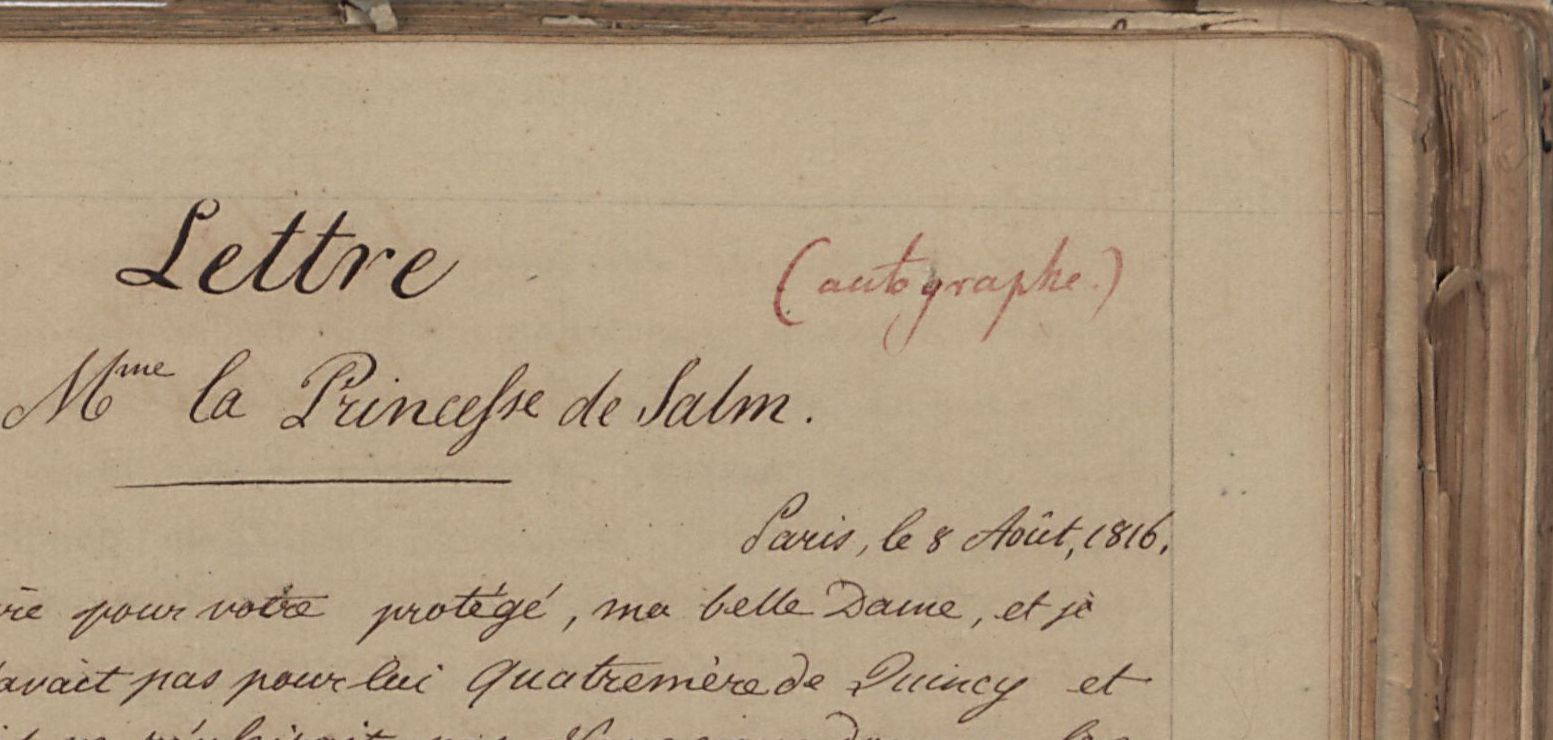
\includegraphics{img/CdS02_Konv002-02_0064_detail.jpg}
					\caption{Rubrique "autographe".}
					\label{autographe}% Le label est le Fig. qui se place au début de la légende, le premFig est la clé d'appel de la figure.
				\end{figure}
			\end{itemize}

			
			Il pourrait être pertinent de reprendre ou de créer d'autres concepts :
			\selectlanguage{english}
			\begin{itemize}
				\item \textbf{Note}: \langue{pour les notes infrapaginales (utilisé dans SegmOnto pour les imprimés\selectlanguage{french}\footcite{Imprimes2021}}
				\selectlanguage{english}
				\item \textbf{Postscritp}: \langue{cela repmplacerait le rôle à l'origine assigné à \langue{Additions}. J'opterais bien pour le jaune car il ne va pas me servir par ailleurs, et qu'on ne risque guère d'avoir un tampon proche du post-scriptum}.
				
			\end{itemize}
			\selectlanguage{french}
			
			La figure \ref{typageRegions} \hyperref[typageRegions]{ci-dessous} propose une mise en oeuvre de ce typage des régions.	

	        \begin{figure}[!h]
	        	% !h ancre l'image dans le flux de texte, sinon elle va n'importe où !
	        	\centering
				\rotatebox{90}{%
					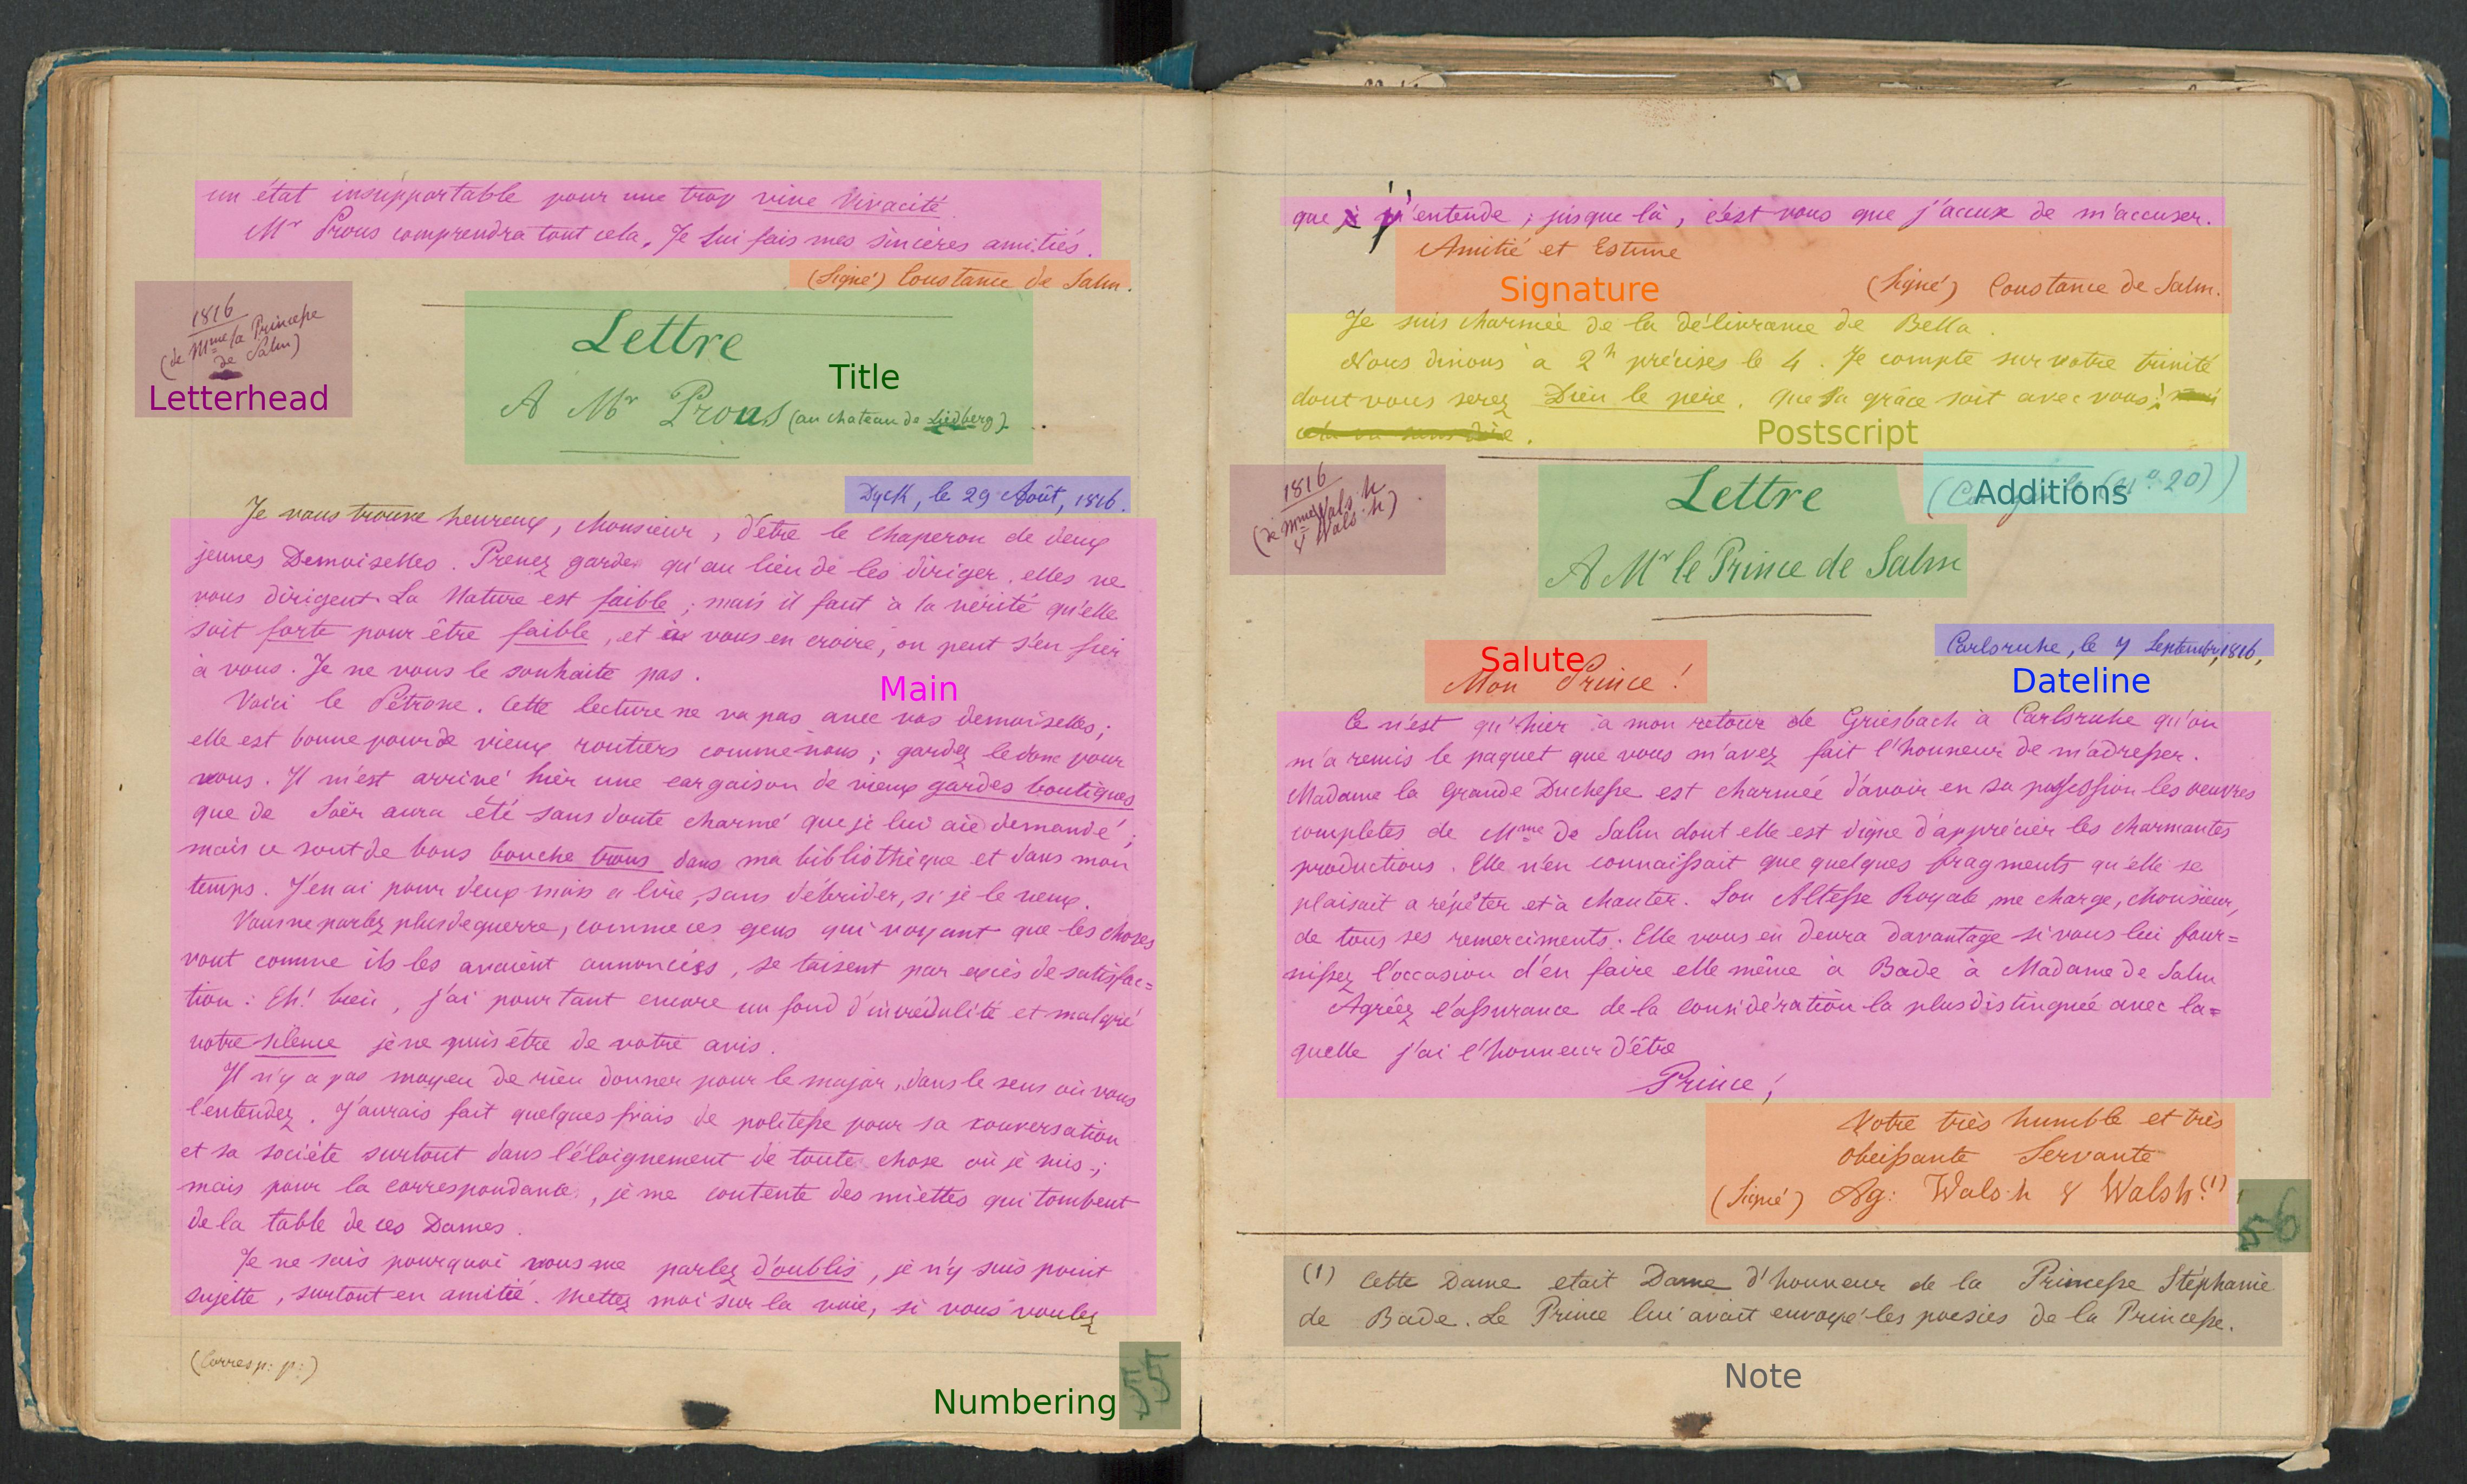
\includegraphics[scale=0.65]{img/essai-zones-CdS02_Konv002-02_0066.jpg}%
				}%
			\caption{Exemple de typage des zones de texte sur une double page.}%
			\label{typageRegions}%
	        \end{figure}
        
            \subsection{Typer les lignes d'écriture}
            Les types de lignes dont on propose l'utilisation sont~:
            
            \begin{itemize}
				\item \textbf{Main}
				\item \textbf{Verse}: \langue{les passages en vers sont relativement nombreux}
				\item \textbf{Correction}: \langue{catégorie existant par défaut dans e-Scriptorium, elle s'appliquerait uniquement pour les corrections appliquées dans l'interligne.}
            \end{itemize}
        
	        \subsection{Phénomènes graphiques particuliers}
            \gls{cds} a corrigé certains mots de sa main~:
 
				\begin{itemize}
				 	\item En rayant une lettre, un mot ou plusieurs mots, ou bien en réécrivant par dessus le texte. Dans de nombreux cas cela consiste en une simple lettre barrée~; le typage de la ligne demanderait alors beaucoup d'effort pour un résultat minime~;
				 	\item En réécrivant dans l'interligne~: il est alors pertinent d'utiliser le type de ligne e-Scriptorium \textbf{Correction}.
				\end{itemize}
			
			Un ensemble de solutions d'encodage des corrections a été proposé dans le cadre du projet DAHN\footcite{chiffoleauFewTipsReading}. J'envisage plutôt \textbf{ne pas encoder ces éléments dans la phase d'HTR}, et de ne les aborder que la phase d'édition. Il sera de toute façon necessaire, lors de la reprise manuelle de l'édition TEI, de suivre la reproduction du manuscrit à éditer. En outre, introduire des caractères tels que £, €, etc. dans la transcription génèrerait du bruit dans l'entraînement du modèle HTR et imposerait une phase de nettoyage pour les réutilisations éventuelles des vérités de terrain.
			
			En somme, il s'agirait de \textbf{transcrire tout ce qui est lisible} (y compris les lettres biffées, lorsque c'est possible), en privilégiant le dernier état du texte dans le cas où la correction a été superposée à la première couche d'écriture.
			
		\section{Mise en oeuvre de la reconnaissance d'écriture}
			Dans le cadre de son stage, H.~Souvay a initié l'entraînement d'un modèle HTR à partir d'un petit volume de vérités de terrain \footcite{souvayCorrespondanceConstanceSalm2021}. La méthodologie employée était la suivante~:
			\begin{quotation}
				Nous avons décidé de tenter la transcription automatique sur un sous-ensemble du corpus composé de copies de lettres compilées dans des recueils. […] Les mains sont relativement constantes dans le temps dans ce sous-ensemble contrairement au reste du corpus. Même proches, ces mains demeurent différentes. Nous avons donc opté pour l’entraînement d’un modèle multi-mains, c’est à dire un modèle non-spécialisé capable de transcrire plusieurs mains représentées dans le corpus d’entraînement\footcite[p.~6-7]{souvayCorrespondanceConstanceSalm2021}
			\end{quotation}

			Il s'agit dans un premier temps d'augmenter le volume des vérités de terrain pour améliorer les performances du modèle entraînés par H. Souvay.
			
			L'objectif visé est de dépasser un taux de précision de reconnaissance de 90\% pour chaque main.
	
		\section{Automatiser la correction des prédictions}
			Les corrections à appliquer aux prédictions \gls{htr} sont nombreuses. Il s'agit d'un travail conséquent à mener avec prudence. Le risque de son automatisation est notamment de remplacer involontairement des prédictions justes ou de remplacer des prédictions fausses par d'autres prédictions fausses. Le contrôle des propositions automatiques de correction est donc nécessaire, bien qu'un trop grand nombre de données à contrôler puisse nuire gravement à la rentabilité du processus.
			
			L'automatisation de la correction des prédictions a pour objectif d'accélérer le passage de la prédiction au format XML-TEI. Le résultat de cette correction est imparfait~; par conséquent cette correction n'intervient pas dans le processus d'entraînement d'un modèle \gls{htr} qui dépend de transcriptions les plus justes possibles. Une fois les modèles \gls{htr} correctement entraînés, la correction automatique permet de résoudre rapidement un certains nombres d'erreurs en amont la transformation au format TEI, où une correction manuelle approfondie du texte est nécessaire pour son établissement définitif.
			
			Nous avons suivi la démarche explicitée dans la documentation du projet DAHN\footcite{chiffoleauHowPostOCRCorrection2022} et proposé quelques développements aux scripts issus de ce projet.
			
			\subsection{Champ d'application et limites}	
				La correction automatisée se concentre sur l'orthographe des mots. Elle n'aborde pas la ponctuation et s'appuie sur des dictionnaires où l'accentuation des mots est normalisée selon l'usage moderne (alors que l'édition finale doit respecter l'usage scribal). Enfin, elle ne traite pas le problème des mots mal prédits dont l'orthographe est attestée ailleurs dans les vérités de terrain~; par exemple, dans la prédiction \textit{Dans \textbf{vu} siècle où tous les talens…}, la prédiciton erronée \textit{vu} pour \textit{un} ne sera pas corrigée car le mot \textit{vu} est attesté ailleurs\footnote{Nous avons tenter l'automatisation de ce type de correction, mais considérant qu'il impose de passer en revue tous les mots dont l'orthographe est déjà attestée ailleurs dans nos vérités de terrain, cette opération fait perdre plus de temps qu'elle n'en fait gagner.}.
					
			\subsection{Analyser les mots}
				Nous avons appliqué le script d'analyse de mots \textsf{spellcheck-texts.py}\footcite{biaySpellcheckTextsPy2022} à nos prédictions HTR\footnote{Ce script est fondé sur l'utilisation du module publié par  \cite{barrusPyspellcheckerPurePython}. Celui-ci procède à une recherche de correspondances entre les formes du texte et un dictionnaire de référence par des permutations de lettres~: il est en mesure de proposer des formes considérées comme justes dans une limite de deux fautes par mot\footnote{Par exemple, il reconnaît que la meilleure proposition pour le mot \textit{deusx} est \textit{deux}, mais n'est pas capable d'associer la forme \textit{pubièes} aux mots de la famille de \textit{publier}}}.
						
				Afin de faciliter la correction des dictionnaires générés par le script pour chaque page (chaque proposition de correction doit en effet être contrôlée), on a développé ce script pour afficher le contexte du mot et en conserver la mémoire, ce qui limite un peu les allers-retours entre le dictionnaire à corriger et l'image ou la prédiction d'origine.
				
				Dans le but d'optimiser la performance de l'analyse des mots on a développé une fonction appelée \textsf{collecteMots}, qui fouille les vérités de terrain déjà constituées et permet de valider automatiquement les mots déjà rencontrés dans le traitement de la correspondance de \gls{cds}, évitant ainsi une recherche plus coûteuse dans un dictionnaire généraliste de la langue française, évitant également le contrôle de ces mots par l'éditeur.
				
				Les corrections précédemment validées sont, elles aussi, mobilisées lors de l'analyse des prédictions, ce qui permet de réexploiter facilement des corrections.
				
				Les corrections s'avérant nombreuses, le script \textsf{textCorrection.py}\footcite{biayTextCorrectionPy2022} écrit par F.~Chiffoleau a dû être perfectionné afin de procéder à une tokénisation des mots, pour corriger avec exactitude les formes erronées présentes dans le texte. Nous avons pour cela utilisé le module Spacy\footcite{SpaCyIndustrialstrengthNatural}.
								
			\subsection{Gérer les résolutions ambiguës}
				Appliquer des scripts de correction automatique, on l'a signalé plus haut, comporte le risque d'appliquer partout des corrections ne se justifiant que dans certains cas et ainsi de générer des fautes. Le problème de l'ambiguïté des corrections se pose lorsqu'une prédiction peut se prêter selon le contexte à plusieurs résolutions différentes~: par exemple \textit{cele}, qui peut résulter tantôt de l'oubli d'un \textit{l} (on corrigera en \textit{celle}), tantôt de la reconnaissance d'un \textit{e} à la place d'un \textit{a} (on corrigera en \textit{cela}).
							
				Dans un premier temps nous avons procédé selon une méthode d'automatisation qui neutralisait les corrections ambiguës~: \textit{cele} était intégré à la liste globale des corrections avec une absence de lemme afin d'être exclu de la correction automatique.
				
				Cette méthode présentait plusieurs inconvénients~:

				\begin{itemize}
					\item Une fois que l'on avait procédé à des corrections pour les mots d'une page, le script qui les intégrait au fichier rassemblant toutes les corrections contrôlait qu'une forme ne puisse pas être associée à plusieurs corrections. Lorsqu'une ambiguïté était repérée, il fallait intervenir sur les deux fichiers pour neutraliser la correction. Devenu fréquent, ce processus diminuait le bénéfice de temps attendu de la correction automatique~;

					\item D'autre part, il s'est avéré que les corrections ambiguës sont nombreuses, car il suffit d'une faute sur un petit mot pour le rendre ambigu avec un autre mot~: \textit{uue} peut être corrigé en \textit{rue} ou en \textit{une}~; \textit{veus} peut être corrigé en \textit{veux} ou en \textit{vous}~; \textit{ceste} peut être corrigé en \textit{cesse} ou en \textit{cette}.
				
				\end{itemize}
				
				Plutôt que de neutraliser la correction de ces mots, il s'est donc avéré nécessaire de prendre en charge ces ambiguïtés.
				
				Il fallait pour cela résoudre une nouvelle difficulté~: opérer des corrections automatiques sur de petits mots fréquents a rendu nécessaire l'application des corrections au niveau de chaque ligne d'écriture, car les appliquer à une page entière aurait sans doute entraîné des corrections erronnées.
						
				Afin de faciliter la sélection de la bonne correction parmi une liste de propositions, on a par écrit une nouvelle fonction (\textsf{ordreOccurrences}) dont le rôle est de classer les mots attestés dans les vérités de terrain par ordre décroissant de nombre d'occurrences. Ainsi, le mot le plus fréquent est toujours proposé comme premier choix au correcteur.
			
	\appendix
	
	\renewcommand{\appendixpagename}{Annexes}
	% Pour renommer en "Annexes" la page de titre "Appendices"
	
	\renewcommand{\appendixtocname}{Annexes}
	% Pour renommer en "Annexes" le nom des annexes dans la table des matières
	
	\addappheadtotoc% Ajoute les annexes à la table des matières
	
	\appendixpage % Crée une page de titre pour les annexes
	\chapter{Normes de transcription}
	
		\section{Accentuation}
		L'usage des accents a été normalisé selon les règles modernes.
		
		\section{Majuscules et minuscules}
		La casse a été respectée sans appliquer les règles modernes~: \textit{je lis les Journaux Allemands}.
		
		\section{Coupure des mots}
		La coupure des mots a été respectée~: \textit{d'avantage, Ç'a été}.
		
		Nous n'avons pas restitué de trait d'union lorsque l'usage moderne l'imposerait~: \textit{portez vous bien}.
				
		\section{Orthographe}
		L'orthographe des mots a été respectée~: \textit{enfans, momens, sentimens, cahos}.
		
		\section{Abréviations}
		Les abréviations ont été transcrites sans être résolues~: \textit{9bre} pour novembre.

		\section{Ponctuation}
		Les signes de ponctuation ont été transcrits fidèlement.
		
		\section{Corrections}
		On transcrit tout ce qui est lisible, y compris les lettres biffées, lorsque c'est possible. On privilégie le dernier état du texte dans le cas où la correction a été superposée à la première couche d'écriture.
		
		Lorsque l'orthographe est erronée, on transcrit le mot sans le corriger~: \textit{Mr Prons} pour \textit{M. Prous}.
           	
	% Bibliographie
	\printbibheading[heading=bibintoc]%Pour afficher seulement le titre général de la bibliographie
	\printbibliography[heading=subbibliography, title=Scripts, keyword=scripts]

\end{document}